% superlight clients
% sidechains
\section{Our Contributions}
\subsection{Superblocks and NIPoPoWs}

We create a decentralized blockchain client or verifier which, having only
\emph{genesis}, connects to multiple provers, at least one of which is honest,
is able to ascertain the confirmation of a transaction. Using its full local
chain, each prover generates a succinct proof and sends it to the verifier.
Adversarial provers can send anything in the place of a proof. By comparing the
proofs in terms of the amount of proof-of-work they encode, the verifier deduces
which blockchain contains the most proof-of-work without receiving and
validating every block header. The proofs the provers send are only generated
once and do not require multiple interrogation questions from the verifier. As
such, these proofs are non-interactive and we call them \emph{Non-Interactive
Proofs of Proof-of-Work} (NIPoPoWs).

To create such succinct representations of work, we look at the distribution of
block hashes in the chain. Every valid block $B$ satisfies the proof-of-work
equation $H(B) \leq T$ where $T$ is the mining target, but some blocks satisfy
it better than others. Some blocks so happen to have a hash with value
\emph{much} lower than $T$, even though this is not required for validity and is
not intentional. For example, some blocks will satisfy $H(B) \leq \frac{T}{2}$.
Concretely, because the hash function is uniformly distributed, in expectation
\emph{half} the blocks will satisfy $H(B) \leq \frac{T}{2}$, a \emph{quarter} of
them will satisfy $H(B) \leq \frac{T}{4}$, an \emph{eighth} will satisfy $H(B)
\leq \frac{T}{8}$, and in general only a $\frac{1}{2^\mu}$ fraction of blocks
will satisfy $H(B) \leq \frac{T}{2^\mu}$. If a block satisfies this inequality
for some $\mu \in \mathbb{N}$, we say that it is of \emph{level} $\mu$ and call
it a $\mu$-superblock (and note that a $\mu$-superblock for $\mu > 0$ is also
a $(\mu - 1)$-superblock). The probability of a valid block $B$ being a
$\mu$-superblock is:

\[
\Pr[H(B) \leq \frac{T}{2^\mu}|H(B) \leq T] = \frac{1}{2^\mu}
\]

Under this light, the blockchain looks as illustrated in
Figure~\ref{fig.superblocks}. Of course, because block hashes behave randomly,
this image will be probabilistic and blocks may not be precisely distributed as
expected.

\begin{figure}[ht]
    \caption{Superblocks distributed within a blockchain.
    Higher levels have achieved a higher difficulty during
    mining.}
    \centering
    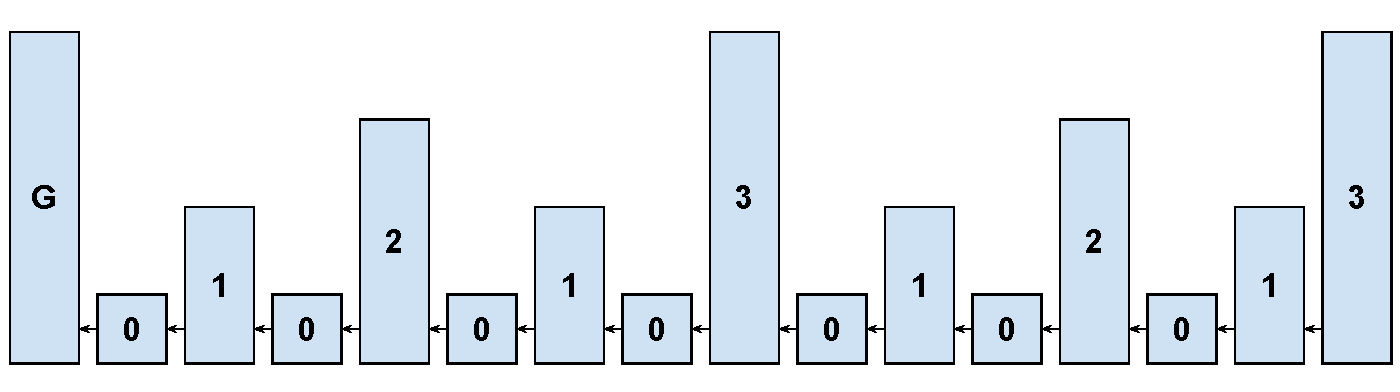
\includegraphics[width=0.7\columnwidth,keepaspectratio]{chapters/introduction/figures/superblocks.pdf}
    \label{fig.superblocks}
\end{figure}

When a chain $\chain$ is mined, there will therefore exist a subsequence of
it, consisting only of blocks of level $\mu$, which is going to be only
$\frac{|\chain|}{2^\mu}$ blocks long. The core idea of the construction is this:
Instead of sending the full chain, the prover chooses a level $\mu$ and sends
this as a \emph{representative of the underlying work}. Presenting a block of
level $\mu$ captures the fact that work of about $2^\mu$ has happened around it
without presenting that work itself. As such, a superblock is a way for the
prover to \emph{sample} the blockchain in a way that can convince the verifier:
When the verifier receives $m$ blocks of level $\mu$, it can deduce that
approximately $m 2^\mu$ regular blocks must exist around those superblocks.
Constructions based on this simple idea instantiate NIPoPoWs by leveraging
superblocks and we call them \emph{superblock NIPoPoWs}.

A simplified description of our protocol then works as follows. Initially, some value
$m$ is fixed, representing the number of blocks that the verifier wishes to
receive to feel safe. This $m$ is a constant parameter. The honest prover then
chooses the highest level $\mu$ which has at least $m$ blocks at that level.
Choosing any level above $\mu$ would not satisfy the verifier, as fewer than $m$
blocks would be transmitted. Choosing any level below $m$ would be wasteful, as
more blocks would have to be transmitted. This prover choice is illustrated in
Figure~\ref{fig.level-threshold}. Suppose that the verifier receives two
proofs from two provers, one of which is honest while the other adversarial, and
wishes to compare them. The verifier first checks that all the blocks it has
received really are $\mu$-superblocks by verifying the proof-of-work equation
parameterized by $\mu$ is satisfied, and that each proof it has received has at
least $m$ blocks. Then, just as an SPV verifier would compare the length of two
full chains, the NIPoPoW verifier now simply \emph{counts} the number of blocks
it has received from the two provers and announces that the one with the most
blocks is the winner. If the verifier receives the proofs $\pi_1$ and $\pi_2$,
then the decision is simply the result of the comparison $|\pi_1| > |\pi_2|$.

\begin{figure}[ht]
    \caption{A superblock NIPoPoW prover chooses the threshold (dashed line)
    corresponding to level $\mu = 2$ for the verifier requirement $m = 4$.}
    \centering
    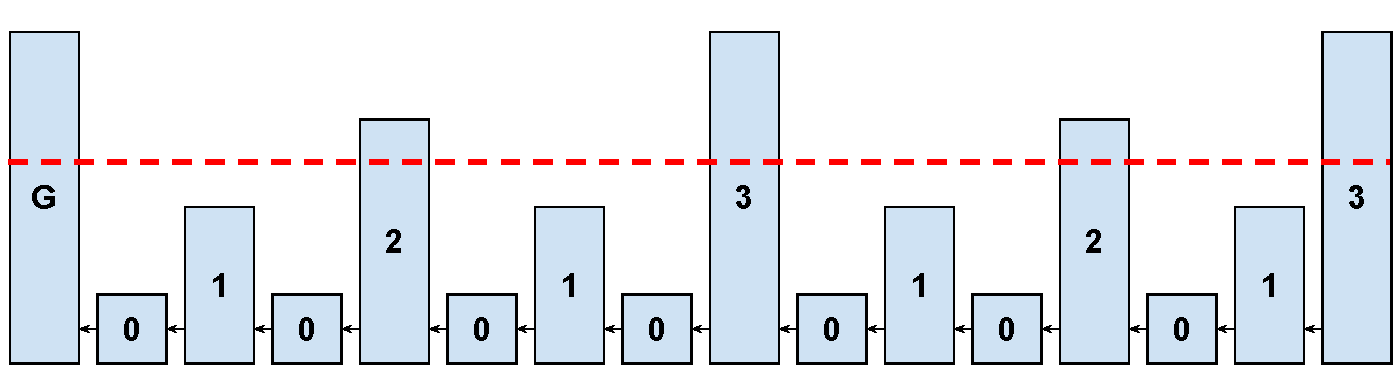
\includegraphics[width=0.7\columnwidth,keepaspectratio]{chapters/introduction/figures/level-threshold.pdf}
    \label{fig.level-threshold}
\end{figure}

The crucial point in terms of security is that an adversary cannot fake this
set of superblocks without actually putting in the work. An adversary that
produces a $\mu$-superblock will also in expectation generate some $2^\mu$
regular blocks in the process (even though the adversary may of course choose
to discard these). Because the adversary has minority mining power, an adversary
cannot create a longer sequence of $\mu$-superblocks faster than the honest
parties create one, for the same reason that an adversary cannot create a longer
regular blockchain faster than the honest parties create one.

Let us count how many different levels $\mu$ there are in a chain. If the chain
has length $|\chain|$, then going up to level $1$ cuts the chain in half, and we
expect to see only $\frac{|\chain|}{2}$ superblocks of level $1$. Moreover, this
continues with subsequent increases in level, until at level $\mu =
\log|\chain|$ we expect to find only $\frac{|\chain|}{2^\mu} = 1$ block. As soon
as we get to level $\log|\chain| + 1$, we expect to find no more blocks of that
level or above. The number of levels is therefore $\log|\chain|$.

To ensure that the blocks sent by the prover cannot be reordered in the wrong
chronological order, just as in the regular underlying blockchain, we need to
introduce pointers that point between consecutive blocks of the same level. As
such, a $\mu$-superblock must include in its contents a pointer to the most
recent $\mu$-superblock that was mined before it. Unfortunately, we cannot add
just these exact pointers to the block contents, because the pointer data must
be included in the contents that are hashed during the attempt to find
proof-of-work. It seems that we must predict what level a block will have prior
to it being mined, but its level depends on its hash, which is a product of its
mining. Therefore, we will simply include all the pointers that could be needed
regardless of what level the block achieves. Prior to mining any block, the
miner collects a pointer to the most recent superblock of each level it has seen
so far. It places these pointers in a list which it then includes in the block
it is mining. When the block is mined, regardless of what level it achieves, it
will have a pointer to the most recent block of its own level.

The number of pointers that need to be included in this manner is small because
the number of levels the blockchain will ever reach is $\log|\chain|$. This
interlinking is illustrated in Figure~\ref{fig.hierarchy}. To avoid premining of
superblocks (blocks that were mined prior to the creation of the genesis block),
we require that the interlink vector of every block also contains a pointer to
the genesis block. By having miners add these extra pointers to blocks, the
verifier can check that the blocks in each proof presented have been mined in
the order given. We see that NIPoPoWs are \emph{subchains} of the blockchain in
that they form subsequences of the block sequence and also maintain pointers
across. The change of adding interlink pointers seems on the surface to require
that miners change their behavior and so a hard fork (a breaking change of
consensus protocol rules) is required. However, the upgrade can be deployed
using a soft fork (a backwards-compatible change), or even without requiring any
miner upgrade in what we introduce as a \emph{velvet fork}.

\begin{figure}[ht]
    \caption{The interlinked blockchain. Each superblock is drawn taller
    according to its level. A new block links to all previous blocks that
    have not been overshadowed by higher levels in the meantime.}
    \centering
    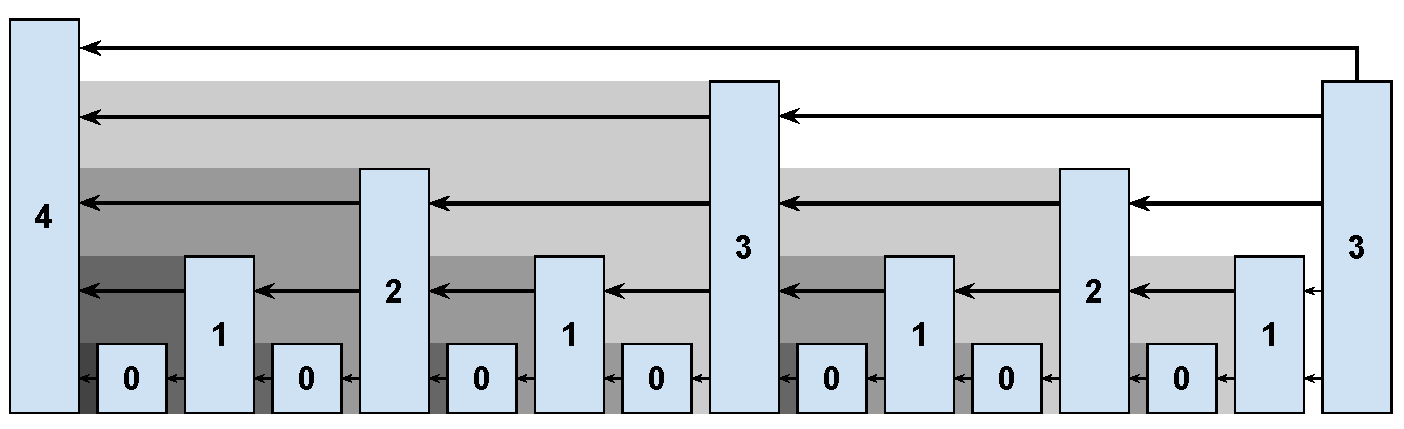
\includegraphics[width=0.9\columnwidth,keepaspectratio]{chapters/introduction/figures/level-shadows.pdf}
    \label{fig.hierarchy}
\end{figure}

Because the two provers may send chains of different levels, it may be necessary
for the verifier to compare the two proofs according to different levels. For
this purpose, the verifier weights the proofs according to their level prior to
comparison. The result of the comparison is then
$2^{\mu_1}|\pi_1| > 2^{\mu_2}|\pi_2|$, where $\mu_1$ and $\mu_2$ indicate the
level of proofs $\pi_1$ and $\pi_2$ respectively. If the two proofs are at the
same level, this comparison reduces to a simple comparison by count. We term
this comparison which can happen \emph{across} levels the \emph{charity}
construction. As we will see in later chapters, the verifier can choose to
compare the two proofs at a common level, simplifying the construction, albeit
to some loss in security. We term the construction which compares across a
common level the \emph{distill} construction.

\subsection{Comparing NIPoPoWs}
While the protocol we have presented so far works \emph{in expectation} against
any adversary, we want to design a protocol that also works \emph{with
overwhelming probability}.  Let us now discuss the role of the security
parameter $m$ that the verifier requires for safety. The property we can prove
from the honest majority assumption is that, in a given period of time that is
sufficiently long, the honest miners mining on their regular $0$-level chain
will generate more $\mu$-superblocks than an adversary with any mining strategy.
This ``sufficiently long'' period of time is ensured by the $m$ security
parameter that the verifier requires. If any of the two superchains consists of
at least $m$ superblocks, this must necessarily have required a long time to
generate as long as $m$ is sufficiently large (in later chapters, this will be
made precise with a Negative Binomial Chernoff bound). If a sufficiently long
time has passed, the length of the superchains will be close to their
expectations and correspond to the mining power of the adversary and the honest
parties respectively (this will later be made precise with a Binomial Chernoff
bound). Because the adversary has minority mining power, their superchain will
be shorter with overwhelming probability. As we increase the parameter $m$ to
some reasonable value (say $m = 128$), the probability that an adversary is able
to attack our protocol drops exponentially in $m$ (according to a function
asymptotically similar to $2^{-m}$).

If the honest and adversarial verifiers send chains that share some blocks,
there is some probability that the adversary is able to convince an honest
verifier of an invalid claim. What we wish to ensure is that the honest NIPoPoW
verifier will never be made to disagree with a corresponding SPV verifier. For
the argument outlined above to hold, we must ensure that the verifier requests
from the two provers at least $m$ superblocks that are \emph{distinct} in each
of their proofs. This ensures the adversary will not be able to reuse blocks
from the honest chain in her proof. Towards this purpose, the verifier asks the
two provers to choose a level $\mu$ such that there are at least $m$ blocks in
each of their proofs \emph{after} the most recent block shared among their
chains (the \emph{lowest common ancestor block} or \emph{LCA block}) as
illustrated in Figure~\ref{fig.lca-comparison}.

\begin{figure}[ht]
    \caption{A comparison across two chains sharing an LCA. The comparison must
    be performed on the independent subchain suffixes after the highlighted block.}
    \centering
    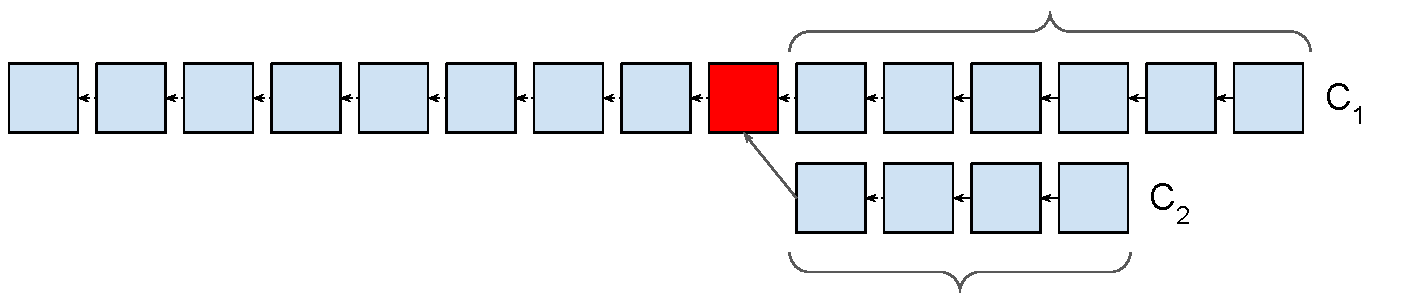
\includegraphics[width=0.9\columnwidth,keepaspectratio]{chapters/introduction/figures/lca-comparison.pdf}
    \label{fig.lca-comparison}
\end{figure}

This can be solved by introducing interactivity in a protocol that works as
follows. Initially, both provers send their highest level $\mu$ that has at
least $m$ blocks to the verifier. The verifier inspects both proofs and finds
their LCA block $b$. He then sends the LCA back to the provers and requests more
information. Each prover subsequently finds the highest level $\mu'$ that has at
least $m$ blocks \emph{after block} $b$. He sends all blocks of level $\mu'$ that
follow $b$. The verifier again inspects the two
proofs and finds their new LCA block $b'$. The process continues until one of the
two provers is not able to keep up with the interrogation. The number of
interrogation steps will be logarithmic, as they are bounded by the number of
levels. Because there can be
no two chains at level $0$ which are both long and significantly diverge, one of
the two provers will necessarily fail.

While it seems that this requires some interactivity, in reality the provers can
provide sufficient evidence upfront so that no interrogation is needed and the verifier can compare proofs
completely
offline. The prover must ensure that there are sufficient blocks in the proof to
enable a comparison regardless of which block is deemed to be the LCA block (as
the adversary can create a proof which essentially chooses the LCA in her
favour). As such, no matter what block in his proof is chosen as the LCA block
$b$ after which the comparison will be performed, the honest prover wants to
ensure he will be successful. The prover includes sufficient blocks so that for
every block $b$ in his proof (a candidate LCA), there exists some level $\mu$
for which at least $m$ superblocks of that level will appear after $b$.
Furthermore, to ensure no work is missed, the honest prover wants \emph{all} his
blocks of the chosen level to appear after $b$.

This requires us to build a prover that sends blocks at multiple levels. A
summary of the construction is then as follows. The prover first chooses the
highest level $\mu$ which has at least $m$ blocks. He sends all
$\mu$-superblocks. Then, for each lower level $j - 1$, he sends sufficient
blocks of level $j - 1$ to cover the same range that the last $m$ blocks of level
$j$ span. The blocks that are selected for sending in such a NIPoPoW are
illustrated in Figure~\ref{fig.nipopow-example}. In this example, the protocol is
working with parameter $m = 3$. Initially, the prover chooses the \emph{highest}
level $\mu$ that has at least $m = 3$ blocks. In this case, he selects $\mu = 2$
which has $4 \geq m$ blocks, as level $3$ would be insufficient with only $2 <
m$ blocks. All $4$ blocks of $\mu = 2$ are included. Subsequently, the last
$m = 3$ blocks of level $\mu = 2$ are considered and the $6$ blocks of level $1$
that span the same range are also included. Lastly, the last $m = 3$ blocks of
level $\mu = 1$ are considered and the last $6$ blocks of level $0$ that span the
same range are also included. The final proof is $10$ blocks long (because some
blocks belong to multiple levels, but do not need to be repeated in the proof).

\begin{figure}
    \caption{
      A Non-Interactive Proof of Proof-of-Work based on superblocks. Multiple
      squares stacked above one another illustrate the same block which spans
      multiple superblock levels. The solid blocks are included in the proof.
      The dashed blocks are not selected for proof inclusion at that level.
    }
    \centering
    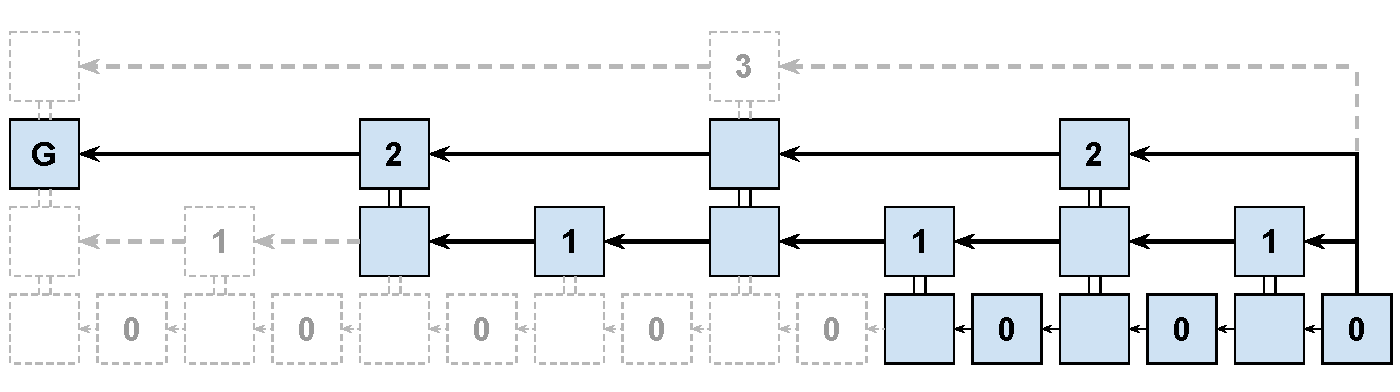
\includegraphics[width=\columnwidth,keepaspectratio]{chapters/introduction/figures/non-interactive-popow.pdf}
    \label{fig.nipopow-example}
\end{figure}

To compare two proofs $\pi_1$ and $\pi_2$ of this style, the verifier first
finds the LCA block $b$ among them. He then chooses a level $\mu$ such that at
least one of the provers has provided $m$ blocks of level $\mu$ after $b$ and
compares the count of distinct blocks at that level. Once we introduce our full
chain traversal notation, this comparison can be expressed elegantly using the
inequality

\[
|\pi_1\{b{:}\}\upchain^\mu| > |\pi_2\{b{:}\}\upchain^\mu|
\,.
\]

Even though multiple levels have been included in the proof, the proofs only
take logarithmic size and are therefore succinct. The reason is that the number
of levels is logarithmic, while the number of blocks included in each level is
constant and approximately $2m$ per level, bringing the total to
$2m\log|\chain|$.

\todo{infix}

\subsection{Superlight Mining}
Having created this construction, it is now possible to build \emph{superlight
wallets} that can synchronize exponentially faster than standard SPV wallets.
This still requires provers to be full nodes and have access to a complete
chain. A natural question that arises is whether it is possible to make a
NIPoPoW verifier that has already received a verified NIPoPoW take the place of
a standard prover. The answer is \emph{yes}, because these proofs are
deterministic and can be simply replayed by nodes that have downloaded them.
Additionally, once a NIPoPoW verifier has synchronized with the network, any new
block that is mined on top of the existing chain can also be (fully) verified by
them and adopted by them. Thus, even though the verifier does not hold the whole
chain, it can keep downloading and verifying new blocks from the network. The
next question is whether a verifier who holds a NIPoPoW $\pi$ and receives a
series of new blocks $b_1, b_2, \cdots, b_k$ from the network can convince
another verifier that these blocks now belong to the best chain. This is
possible because superblock-based NIPoPoWs have the \emph{online} property:
Consider a NIPoPoW $\pi$ created for a chain $\chain$. If $b_1$ is created on
top of $\chain$, then it is possible to evolve $\pi$ into a new NIPoPoW $\pi_1$
which pertains to the chain $\chain \concat b_1$ without ever seeing $\chain$.
This is because the new NIPoPoW $\pi_1$ only needs to contain (some) blocks from
$\pi$ as well as $b_1$ itself. This can be used to keep evolving NIPoPoWs as
blocks are added, always only keeping the latest among them. Previous blocks
and old NIPoPoWs can be garbage collected, allowing the node to function with a
state of logarithmic size.

The node that has synchronized using a NIPoPoW and only holds a NIPoPoW can
function as both a prover and a verifier and even be able to deal with cases
of temporary forks. In fact, the node can even \emph{mine} on top of their
NIPoPoW. Because it holds the most recent block of the blockchain, it simply
creates a new candidate block that points to it and attempts to solve
proof-of-work accordingly. If he succeeds, he can broadcast the new block to the
rest of the network and update their local state by evolving their NIPoPoW in
light of the new block. As long as the majority of the mining power is honest,
even \emph{all} miners can upgrade to this logarithmic protocol so that no one
really has to ever save the whole chain. The idea here is that the full history
of transactions is not necessary to achieve economic consensus (i.e., who holds
how much money or how much money remains unspent); what is needed
is to be able to determine whether a new transaction is valid, and for this it
suffices to know the current state of the system, be it unspent transaction
outputs or account balances. This technique, which provides exponential
improvements in the size of state storage, we term
\emph{logarithmic space mining}.

\subsection{Proofs of Proof-of-Stake}
Different techniques can be used to compress consensus state in proof-of-stake
blockchains. Unlike proof-of-work in which the work of a block is a stand-alone
property that can be verified by the verifier, the verification of the
proof-of-stake signature on a block requires the verifier to know the stake
distribution of the current epoch so as to be able to decide whether the key
making the signature corresponds to a correctly elected leader. However, having
the verifier see the whole stake distribution would be inefficient. Instead, we
propose a construction in which the verifier only sees a small sample of the
stake distribution per epoch. The protocol looks at the leaders that were
elected to mint blocks throughout the epoch, and assembles a number of these
leaders into a \emph{committee}. Since the block leaders are selected in a
follow-the-satoshi fashion by respecting the evolving stake distribution, the
committee members are selected in this way too. It has been shown that
committees selected once per epoch in this fashion will have honest majority
\emph{by count} as long as the underlying stake distribution that was used for
the selection process has honest majority by stake.

The light stake verifier looks at one such committee per epoch. For each epoch,
the committee signs off a \emph{certificate} which attests to the election of a
new committee for the next epoch. The committee members themselves are full
nodes who, in the honest protocol, only sign off such certificates attesting to
the correct new committee. The verifier checks that the certificate has been
signed by the majority of an epoch's commitee. By verifying these certificates,
the verifier can ensure that he holds a representative sample of keys for each
epoch. These keys corresponding to the committee of each epoch can then be used
to sign statements alleging that a transaction took place during their
respective epoch. As the verifier knows the committee for each epoch, they can
verify these statements also.

While this construction has eliminated the need for the verifier to maintain the
whole stake distribution as it shifts from epoch to epoch, something that would
require the verifier to look at every transaction, it still requires the
verifier to know a committee for each epoch. These committees can be quite
large to ensure that the sampling of stake is representative. We optimize this
need by introducing the Ad-Hoc Threshold Multi-Signatures (ATMS) primitive, in
which a whole committee is represented by a single short public key. This public
key, called the \emph{aggregate public key}, encodes in it all the public keys
of all committee members, and its size is comparable to a regular public key.
There is one aggregate key per epoch. Furthermore, if multiple committee members
create signatures on a message, these can be \emph{aggregated} into a single
\emph{aggregate signature} which has a small size, comparable to a regular
signature. These signature schemes are also \emph{treshold signatures}:
If a majority of the keys used to create the aggregate public key combine their
signatures into an aggregate signature, the aggregate signature will pass
verification with the corresponding public key in which more keys have been
aggregated. On the other hand, any aggregation of signatures by a minority
number of signatories will not verify. Lastly, the signature scheme is
\emph{ad hoc}, because each member of the committee can locally create their own
signature without interactivity with the rest of the members. The signatures can
then be aggregated by any party, even outside of the signatories themselves.
Similarly, public keys can be generated locally without interactivity and
aggregated later by any party.

The evolution of committees from epoch to epoch is then represented by asking
the verifier to only hold a single aggregate key per epoch. For each transition
from epoch to epoch, the majority of the committee of the previous epoch sign
a certificate transitioning to the committee of the new epoch. The certificate's
text contains the new aggregate public key. These signatures are combined into
an aggregate signature and can be verified by the aggregate public key of the
previous epoch. As such, the verifier simply sees one public key and one
signature per epoch. The aggregate public key of each epoch can also vouch for
events that took place during that epoch such as a particular transaction. For
purposes of synchronization of a light client, the committee corresponding to
the current epoch can vouch for any transactions occurring any time in the past,
and the light verifier can use the current aggregate key to verify any such
claims. The amount of data needed to download is therefore minuscule per epoch.
However, as epochs evolve linearly with time, the asymptotic complexity is still
$\Theta(|\chain|)$, albeit with a very small constant.

\subsection{Sidechains}

Consensus compression is useful for superlight clients and superlight mining.
One of its most interesting application beyond this pertains to cross-chain
communication. Given two chains, the \emph{source chain} and the
\emph{destination chain} which are maintained by independent mining populations,
we want to have the destination chain react to an \emph{event} that took place
in the source chain. The miners on one chain are \emph{isolated} from the other,
and they do not connect to its network. However, users interested in the
cross-chain events can connect to both networks. Because users can be
adversarial, the destination chain miners cannot simply trust the users' claim
that an event took place on the source chain -- it needs to be verified.

Events that can be passed from blockchain to blockchain can be virtually any
predicate pertaining to a small amount of data such as a constant number of
transactions or blocks. In practice, these events can be, for example, about the
fact that a transaction with particular metadata took place on the source
blockchain, that a particular amount has been sent or received, that a
particular account holds a certain amount of balance at some point in time, that
some transaction output remains unspent, that a smart contract method was
called with some particular arguments, or that a smart contract's state
variables held certain values at some point in time.

We create support for cross-chain communication for blockchain systems in which
the source blockchain can produce Non-Interactive Proofs of
Proof-of-Work-or-Stake. As discussed, these systems may need some backwards
compatible upgrades before they can be used as sources, such as introducing
interlinks. On the receiving side, we require the blockchain to either have
native support for consuming these Proofs of Proofs (and its miners to run a
verifier), or to have smart contract support. Smart contract support is
sufficient because a compressed consensus verifier (such as a NIPoPoW or ATMS
verifier) can be written in the code of a smart contract.

The core idea of our sidechain construction is as follows. Whenever an event
takes place within the source blockchain, information about the event as and its
corresponding blockchain is compressed into a Proof of Proof. For proof-of-work
sources, these are NIPoPoWs; for proof-of-stake sources, these are evolving
ATMS. As the proof is a short string, it can be submitted to the destination
blockchain for verification. This verification can be done by the destination
chain miners natively (without ever connecting to the source blockchain), or by
a smart contract. The latter case is the more interesting one, because it allows
blockchains that were never designed to be interoperable to communicate.
In this setting, the code for checking the validity of the NIPoPoW as well
as the code for their comparison is written into smart contract format.
This allows the smart contract running in one blockchain to consume NIPoPoWs
generated about other blockchains. In this case, the miners of the smart
blockchain simply execute the smart contract code as if it were any other smart
contract, without any regard for its
semantics or knowledge that inter-chain communication is taking place.
Once
the smart contract has verified the proof, it may be able to take a decision
immediately (for proof-of-stake sources), or it may need to wait for a short
period to allow for \emph{contesting proofs} to appear (for proof-of-work
sources). In case a fraudulent NIPoPoW pertaining to a shorter chain is
submitted, a contesting proof allows any node monitoring both chains to make
a counter-claim, via a new NIPoPoW, claiming that the original proof was
fraudulent. The smart contract runs the NIPoPoW comparison algorithm and decides
which of the two proofs is the legitimate one. To ensure users have incentives
to submit such proofs, a successful contestation is accompanied by a reward
which is paid out to the contester and is obtained by slashing a collateral
deposited by the original prover. In case no proofs of fraudulence are
submitted, the collateral is returned to the (honest) initial prover.

As we can have both proof-of-work and proof-of-stake sources as well as
proof-of-work and proof-of-stake destinations, this construction allows us to
create communication bridges between any combination of consensus mechanisms.
If the information is passed only one-way, then the communication is
unidirectional. This application is still useful as a mechanism to bootstrap a
new cryptocurrency from an old one. We present one way of doing that by
destroying money on the source blockchain and proving that this happened by
providing a relevant proof submitted to the destination chain. On the other
hand, nothing prevents two blockchains from both functioning as a source and a
destination for each other. This allows us to build fully bidirectional
communication channels between blockchains, giving rise to full two-way pegs.

In a two-way peg, the bidirectional communication can be used to move a coin
from one blockchain to another while it retains its nature, decoupling the
notion of a blockchain from that of a cryptocurrency. The lifecycle of the coin
is as follows. Consider two blockchains A and B and an asset which is natively
issued within chain A. Two smart contracts are deployed for interoperability
purposes, one on chain A and one on chain B. Each of the two smart contracts
records the address of its counterpart. Initially, a coin exists in its native
blockchain A. The coin is locked into a special smart contract within the native
blockchain, which ensures that it cannot be further spent. At this stage,
blockchain A functions as a source blockchain for the communication protocol.
The fact that the coin was locked is proven using a Proof of Proof-of-Work or
Stake. This proof
is created by the user that locked her coin. The proof is submitted to a smart
contract which lives on blockchain B. At this stage, blockchain B functions as a
destination chain. The receiving smart contract verifies the Proof of Proof-of-Work
or Stake and
waits to ensure there is no contestation. At this point, the receiving smart
contract can be certain that the coin was locked into its counterpart which
lives in chain A. Note that the smart contract never directly connected to the
network of chain A. The receiving smart contract mints a new token coin within
blockchain B, equal in nominal value to the value of the locked coin on chain A.
The token on chain B is given the the public key that corresponds to the user
who locked the initial coin on chain A. That token can then be used for exchange
within chain B like a regular currency. However, it is dissimilar from the
native currency of chain B (in fact, chain B may not even have a native currency
of its own, as we will see).

When any user who ends up holding the token within chain B decided to move it
back to chain A, the reverse process is initiated. Chain B now functions as a
source chain, while chain A functions as a destination chain. The token is sent
to the smart contract in chain B. The contract destroys the token. The user who
destroyed their token in chain B then creates a Proof of Proof of this fact.
Again this is a short string which can be submitted to the smart contract that
lives on chain A. The smart contract on chain A verifies the proof attesting to
the destruction of the token on chain B, and waits for potential contestation.
At this point, the smart contract on chain A can be certain that the token has
been destroyed on chain B and can now unlock the corresponding value in native
currency that it currently holds. Because tokens appear on chain B only after
they have been locked in the smart contract of chain A, the smart contract in
chain A will always have sufficient balance to unlock to respond to any
withdrawals.

Lastly, the process is voluntary and any users of A and B who do not wish to use
it do not have to participate or even know about it. Importantly, the miners of
the two chains can remain unaware that the cross-communication is taking place.
Additionally, chain A is \emph{firewalled} from chain B. This means that a
catastrophic failure in chain B, such as an honest majority violation, does not
propagate to chain A beyond the amount of money that was locked in the
cross-chain smart contract. As such, any nodes who are not participating in the
cross-chain protocol will incur no financial losses from such a catastrophic
failure.

\ifdraft
We explore superblocks and the \emph{charity} NIPoPoWs construction in detail in
Chapter~\ref{chapter:work}. We extend them to logarithmic space mining in the
\emph{distill} construction in Chapter~\ref{chapter:superlight}. These two
chapters assume that the target $T$ does not change (the
\emph{static difficulty} setting). We extend our results to the variable
difficulty setting in Chapter~\ref{chapter:variable}.
\fi

\todo{applications to sidechains}

\ifdraft
\todo{Clean up paragraph}
As one application, we give the
construction of a \emph{two-way pegged} asset which can be moved from one
blockchain to another while retaining its nature. We provide a high-level
construction in Solidity. Our construction works across a broad range of
blockchains requiring only two underlying properties. First, that the
\emph{source} blockchain is a proof-of-work blockchain supporting
Non-Interactive Proofs of Proof-of-Work (NIPoPoWs), a cryptographic primitive
which allows constructing succinct proofs \emph{about} events which occur in a
proof-of-work blockchain and which was recently introduced in~\cite{nipopows}.
Support for NIPoPoWs can be introduced to practically any
work-based cryptocurrency such as Bitcoin and Ethereum without a hard or soft
fork. Second, that the \emph{target} blockchain is able to validate such proofs
through smart contracts such as, e.g., Ethereum or Ethereum
Classic.
We give a formal proof of security of our construction via
reduction to NIPoPoW security under the assumption that the interoperating
blockchains are secure individually.
To our knowledge, we are the first to
provide such a construction in
full and prove its security.
\fi

\subsection{Summary of Contributions}
A summary of our contributions and their dependencies, with annotations
indicating where they are presented in this thesis, is visually illustrated in
Figure~\ref{fig.contributions}.

In summary, in this thesis we solve the problem of \emph{consensus compression}
for all decentralized blockchain consensus mechanisms. \textbf{For
proof-of-work}, we introduce the NIPoPoWs primitive (Chapter 3) and we give two
superblock-based constructions of succinct NIPoPoWs protocols in the Backbone
model: First the \emph{charity} construction (Chapter~\ref{chapter:work}), and
second the \emph{distill} construction (Chapter~\ref{chapter:superlight}
and~\ref{chapter:variable}). In the static synchronous model
(Chapter~\ref{chapter:work}), we prove our charity construction with
\emph{goodness} secure against $\frac{1}{2}$ adversaries, but succinct only in
the optimistic setting. Our charity construction \emph{without goodness} as well
as our distill construction are both secure and succinct against $\frac{1}{3}$
adversaries (Chapter~\ref{chapter:variable}). In the synchronous variable model
(Chapter~\ref{chapter:variable}), our distill construction is secure against a
$\frac{1}{3}$ adversary as long as difficulty is non-decreasing. Our charity
without goodness construction is secure against a $\frac{1}{3}$ adversary even
if difficulty is not limited to non-decreasing. Both are succinct as long as
difficulty is not exponentially decreasing. Lastly, in the $\Delta$-bounded
delay setting (Chapter~\ref{chapter:variable}), both constructions are secure
and succinct under the same limitations, but only against a $\frac{1}{4}$
adversary. We give concrete parameter recommendations and run experiments and
simulations indicatively for the charity construction of
Chapter~\ref{chapter:work}. \textbf{For proof-of-stake}, we construct the ATMs
primitive and give signature-based construction (Chapter~\ref{chapter:stake}).
These are secure in the Ouroboros model, but offer only constant improvements
over full clients and hence do not achieve asymptotic succinctness.

We make use of these primitives to build \textbf{cross-chain transfer}
applications, which give rise to interoperability among blockchains, allowing
generic information transfer among work/work, work/stake, and stake/stake
chains. We give the definition of what constitutes a secure sidechain protocol
(Chapter~\ref{chapter:sidechains}) and put forth a cross-chain protocol which we
prove secure. Our protocols can work natively or by leveraging smart contract
functionality. We show how they can be utilized to create one-way and two-way
pegs and discuss several deployment mechanisms which allow them to be deployed
as soft forks or better. Our protocols can also be used to build superlight
clients. Lastly, we show that our proof-of-work protocols specifically can be
utilized to build logarithmic-space miners (Chapter~\ref{chapter:superlight}),
providing exponential improvements over the state and communication complexity
of existing proof-of-work blockchain protocols.

\begin{figure}
    \caption{
      A roadmap of this thesis' structure.
      Our underlying model is shown above the double line.
      Our contributions are shown below the double line and comprise consensus
      compression primitives (above the dashed line) and their applications
      (below the dashed line). The respective chapters are indicated next to
      each topic.
    }
    \centering
    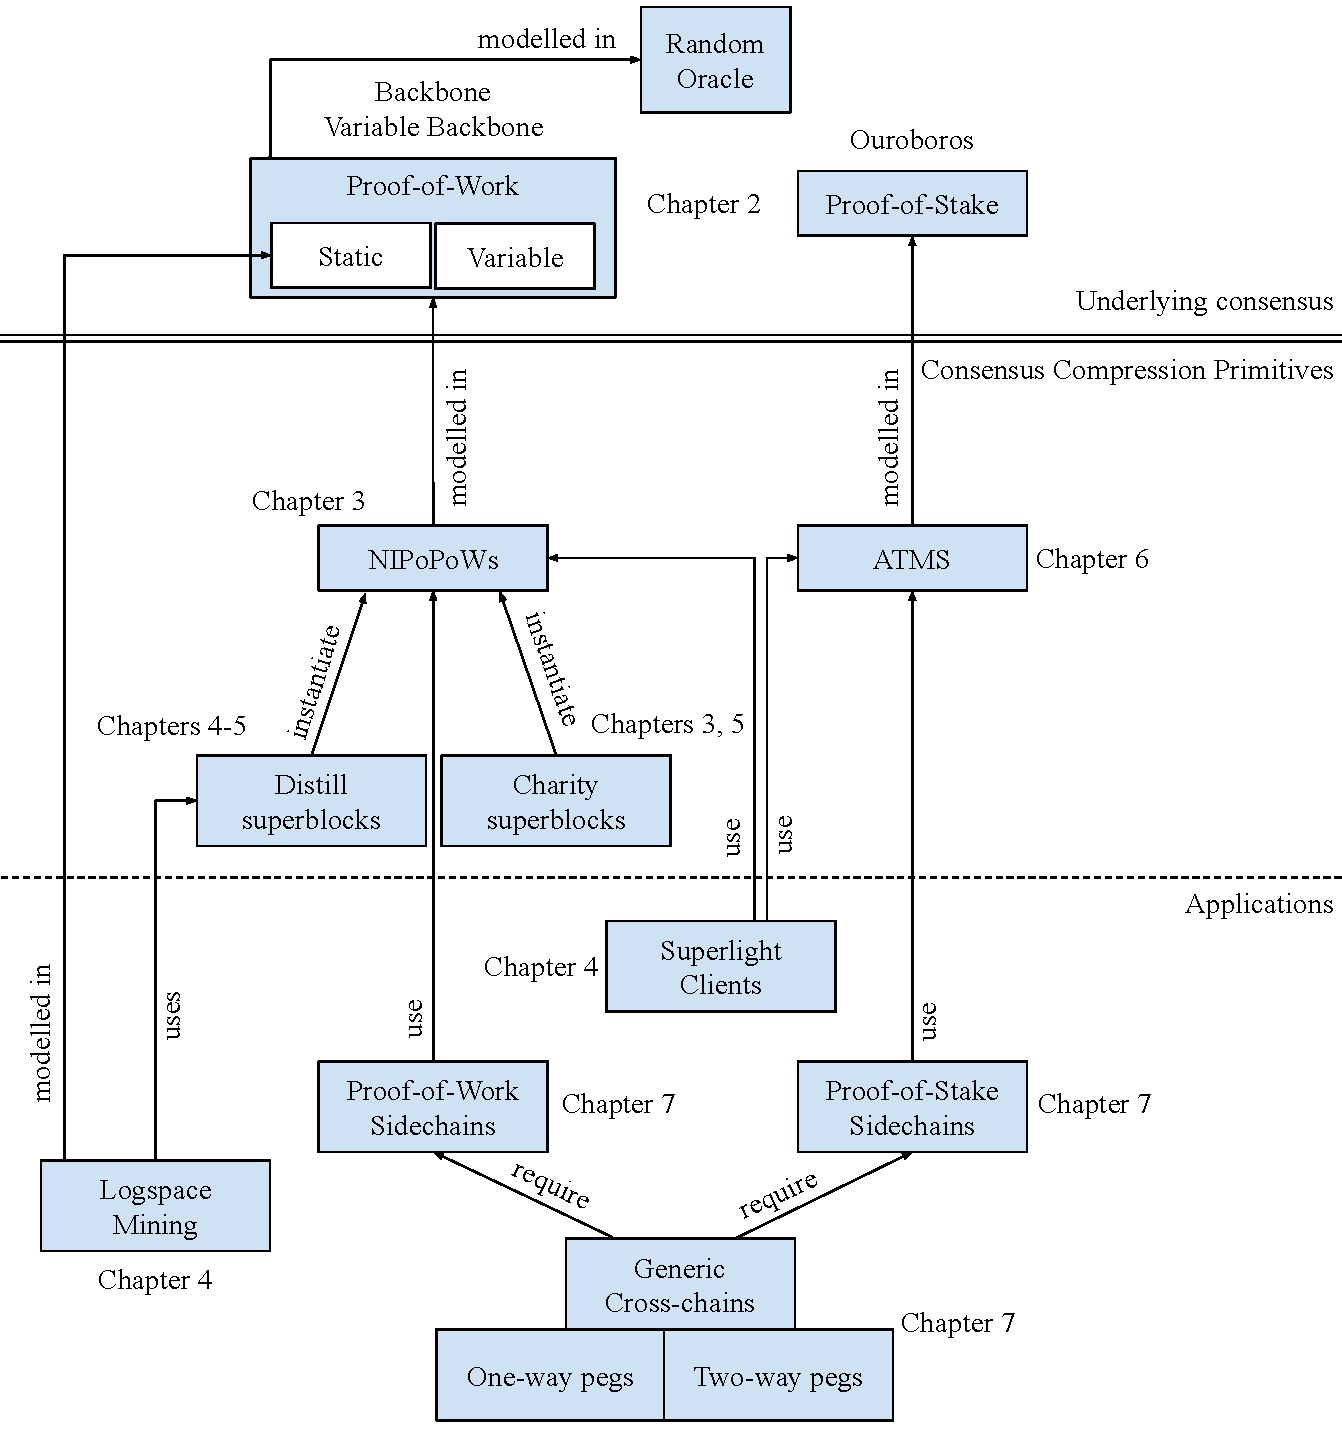
\includegraphics[width=\columnwidth,keepaspectratio]{chapters/introduction/figures/contributions.pdf}
    \label{fig.contributions}
\end{figure}
